\documentclass[a4paper,12pt, oneside]{book}

% \usepackage{fullpage}
\usepackage[italian]{babel}
\usepackage[utf8]{inputenc}
\usepackage{amssymb}
\usepackage{amsthm}
\usepackage{graphics}
\usepackage{amsfonts}
\usepackage{listings}
\usepackage{amsmath}
\usepackage{amstext}
\usepackage{engrec}
\usepackage{rotating}
\usepackage{verbatim}
\usepackage[safe,extra]{tipa}
%\usepackage{showkeys}
\usepackage{multirow}
\usepackage{hyperref}
\usepackage{microtype}
\usepackage{fontspec}
\usepackage{enumerate}
\usepackage{braket}
\usepackage{marginnote}
\usepackage{pgfplots}
\usepackage{cancel}
\usepackage{polynom}
\usepackage{booktabs}
\usepackage{enumitem}
\usepackage{framed}
\usepackage{pdfpages}
\usepackage{pgfplots}
\usepackage{algorithm}
% \usepackage{algpseudocode}
\usepackage[cache=false]{minted}
\usepackage{mathtools}
\usepackage[noend]{algpseudocode}

\usepackage{tikz}\usetikzlibrary{er}\tikzset{multi  attribute /.style={attribute
    ,double  distance =1.5pt}}\tikzset{derived  attribute /.style={attribute
    ,dashed}}\tikzset{total /.style={double  distance =1.5pt}}\tikzset{every
  entity /.style={draw=orange , fill=orange!20}}\tikzset{every  attribute
  /.style={draw=MediumPurple1, fill=MediumPurple1!20}}\tikzset{every
  relationship /.style={draw=Chartreuse2,
    fill=Chartreuse2!20}}\newcommand{\key}[1]{\underline{#1}}
  \usetikzlibrary{arrows.meta}
  \usetikzlibrary{decorations.markings}
  \usetikzlibrary{arrows,shapes,backgrounds,petri}
\tikzset{
  place/.style={
        circle,
        thick,
        draw=black,
        minimum size=6mm,
    },
  transition/.style={
    rectangle,
    thick,
    fill=black,
    minimum width=8mm,
    inner ysep=2pt
  },
  transitionv/.style={
    rectangle,
    thick,
    fill=black,
    minimum height=8mm,
    inner xsep=2pt
    }
  } 
\usetikzlibrary{automata,positioning}
\usepackage{fancyhdr}
\pagestyle{fancy}
\fancyhead[LE,RO]{\slshape \rightmark}
\fancyhead[LO,RE]{\slshape \leftmark}
\fancyfoot[C]{\thepage}


\title{Processo e Sviluppo del Software}
\author{UniShare\\\\Davide Cozzi\\\href{https://t.me/dlcgold}{@dlcgold}}
\date{}

\pgfplotsset{compat=1.13}
\begin{document}
\maketitle

\definecolor{shadecolor}{gray}{0.80}
\setlist{leftmargin = 2cm}
\newtheorem{teorema}{Teorema}
\newtheorem{definizione}{Definizione}
\newtheorem{esempio}{Esempio}
\newtheorem{corollario}{Corollario}
\newtheorem{lemma}{Lemma}
\newtheorem{osservazione}{Osservazione}
\newtheorem{nota}{Nota}
\newtheorem{esercizio}{Esercizio}
\algdef{SE}[DOWHILE]{Do}{doWhile}{\algorithmicdo}[1]{\algorithmicwhile\ #1}
\tableofcontents
\renewcommand{\chaptermark}[1]{%
  \markboth{\chaptername
    \ \thechapter.\ #1}{}}
\renewcommand{\sectionmark}[1]{\markright{\thesection.\ #1}}
\newcommand{\floor}[1]{\lfloor #1 \rfloor}
\newcommand{\MYhref}[3][blue]{\href{#2}{\color{#1}{#3}}}%
\chapter{Introduzione}
\textbf{Questi appunti sono presi a lezione. Per quanto sia stata fatta
  una revisione è altamente probabile (praticamente certo) che possano
  contenere errori, sia di stampa che di vero e proprio contenuto. Per
  eventuali proposte di correzione effettuare una pull request. Link: }
\url{https://github.com/dlcgold/Appunti}.\\
\textbf{Le immagini presenti in questi appunti sono tratte dalle slides del
  corso e tutti i diritti delle stesse sono da destinarsi ai docenti del corso
  stesso}.
\chapter{Metodi Agili}
I \textit{metodi agili} sono stati definiti per rispondere all'esigenza di dover
affrontare lo sviluppo di software in continuo cambiamento. Durante lo sviluppo
si hanno vari passaggi:
\begin{itemize}
  \item comprensione dei prerequisiti
  \item scoperta di nuovi requisiti o cambiamento dei vecchi
\end{itemize}
Questa situazione rendeva difficile lo sviluppo secondo il vecchio metodo
\textit{waterfall} (portando al fallimento di diversi progetti).\\
I \textit{metodi agili} ammettono che i requisiti cambino in modo ``naturale''
durante il processo di sviluppo software e per questo assumono un modello di
processo \textit{circolare}, con iterazioni della durata di un paio di settimane
(figura \ref{agile}). Potenzialmente dopo un'iterazione si può arrivare ad un
prodotto che può essere messo in ``produzione''. Dopo ogni rilascio si
raccolgono \textit{feedback} per poter rivalutare i requisiti e migliorare il
progetto.\\
\begin{figure}
  \centering
  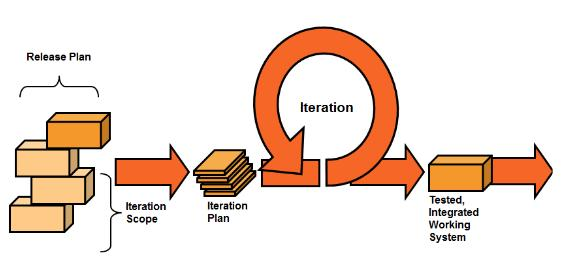
\includegraphics[scale = 0.6]{img/agile.jpg}
  \caption{Rappresentazione grafica del modello agile. I blocchi a sinistra
    rappresentano i requisiti (da sviluppare secondo una certa priorità). Lo
    sviluppo si articola tramite varie iterazioni che porta ogni volta ad
    aggiungere una parte al prodotto finale (ogni iterazione produce, a partire
    da un certo requisito, un parte di
    prodotto di qualità già definitiva, con testing, documentazione
    etc$\ldots$)}
  \label{agile}
\end{figure}
Si hanno quindi aspetti comuni nei metodi agili e nel loro processo:
\begin{itemize}
  \item enfasi sul team, sulla sua qualità e sulla sua selezione
  \item il team è \textit{self organizing}, non essendoci un \textit{manager} ma
  essendo il team a gestire lo sviluppo, dando importanza ai vari membri del
  team
  \item enfasi al pragmatismo, evitando di produrre documenti inutili che
  sarebbero difficili da mantenere, focalizzandosi su una documentazione
  efficacie
  \item enfasi sulla comunicazione diretta e non tramite documenti, tramite
  meeting e riunioni periodiche
  \item enfasi sull'idea che nulla sia definitivo e che non bisogni seguire la
  perfezione fin da subito ma che, ``pezzo per pezzo'', ogni step porterà al
  raggiungimento di una perfezione finale (anche dal punto di vista del design)
  \item enfasi sul controllo costante della qualità del prodotto, anche tramite
  pratiche tecniche come quella del \textit{continuous testing}, dove un insieme
  di test viene eseguita in modo automatico dopo ogni modifica, o anche pratiche
  di \textit{analisi statica e dinamica} del codice al fine di trovare difetti
  nello stesso nonché di \textit{refactoring}
\end{itemize}
\textit{I metodi agili sono molto ``elastici'' e permettono la facile
  definizione di nuovi metodi facilmente adattabili al singolo progetto.}
\section{Scrum}
Tra i vari \textit{metodi agili} uno dei più famosi è \textbf{scrum} (figura
\ref{scrum}).\\
In questo caso la parte di sviluppo e iterazione prende il nome di
\textit{sprint} e ha una durata variabile tra una e quattro settimane, per avere
un rilascio frequente e una veloce raccolta di feedback. I requisiti sono
raccolti nel cosiddetto \textit{product backlog}, con priorità basata sulla base
delle indicazioni del committente. Ad ogni \textit{sprint} si estrae dal
\textit{product backlog} lo \textit{sprint backlog}, ovvero il requisito (o i
requisiti) da implementare nello \textit{sprint}. Lo \textit{sprint backlog}
viene analizzato nel dettaglio producendo i vari \textit{backlog items}, ovvero
le singola funzionalità che verranno implementate nello \textit{sprint}. Si
ottiene quindi di volta in volta un pezzo di prodotto finale, testato e
documentato. Durante le settimane di \textit{sprint} si ha anche un meeting
giornaliero utile per mantenere alti i livelli di comunicazione e visibilità
dello sviluppo. Durante il meeting ogni dev risponde a tre domande:
\begin{enumerate}
  \item Cosa è stato fatto dall'ultimo meeting?
  \item Cosa farai fino al prossimo meeting?
  \item Quali sono le difficoltà incontrate?
\end{enumerate}
l'ultimo punto permette la cooperazione tra team members che sono consci di cosa
ciascuno stia facendo.\\
\begin{figure}
  \centering
  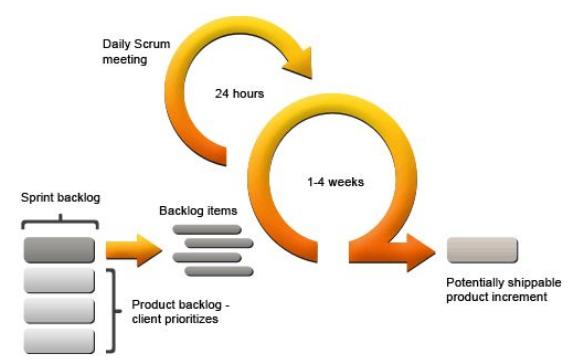
\includegraphics[scale = 0.6]{img/scrum.jpg}
  \caption{Rappresentazione grafica del processo scrum}
  \label{scrum}
\end{figure}
Durante il processo \textit{scrum} si hanno quindi tre ruoli:
\begin{enumerate}
  \item il \textbf{product owner}, il committente che partecipa tramite feedback
  e definizione dei requisiti
  \item il \textbf{team}, che sviluppa
  \item lo \textbf{scrum master}, che controlla che il processo scrum sia svolto
  correttamente
\end{enumerate}
Essi collaborano nelle varie fasi:
\begin{itemize}
  \item product owner e team collaborano nella definzione dei backlog e nella
  loro selezione ad inizio \textit{sprint}
  \item durante lo \textit{sprint} lavora solo il team
  \item nello studio del risultato collaborano tutti coloro che hanno un
  interesse diretto nel progetto (team, product owner, stakeholders) 
\end{itemize}
\textit{Lo scrum master interagisce in ogni fase, fase che viene comunque
  guidata tramite meeting}:
\begin{itemize}
  \item \textbf{sprint planning meeting}, ad inizio \textit{sprint}
  \item \textbf{daily scrum meeting}, il meeting giornaliero
  \item \textbf{sprint review meeting}, in uscita dallo \textit{sprint} per lo
  studio dei risultati
  \item \textbf{sprint retrospective meeting}, in uscita dallo \textit{sprint}
  per lo studio tra i membri del team di eventuali migliorie al processo e allo
  sviluppo del prodotto (anche dal punto di vista delle tecniche e delle
  tecnologie)
\end{itemize}
\section{Extreme Programming}
Un altro tipo di metodo agile è l'\textit{extreme programming} (figura
\ref{extreme}), ormai poco usato. I requisiti prendono i nomi di
\textit{stories}, che vengono descritti come l'utente del sistema, detto
\textit{attore}, che cerca di fare qualcosa tramite una ``narrazione''. Vengono
scelti quindi \textit{stories} per la prossima iterazione, dove si hanno testing
e revisione continua. Le release di ogni iterazione vengono catalogate per
importanza (con anche la solita collezione di feedback). In \textit{extreme
  programming} si hanno davvero molte pratiche:
\begin{itemize}
  \item The Planning Game
  \item Short Releases
  \item Metaphor
  \item Simple Design
  \item Refactoring
  \item Test-First Design
  \item Pair Programming
  \item Collective Ownership (codice condiviso da tutti senza alcun owner, con
  tutti in grado di effettuare modifiche)
  \item Continuous Integration
  \item 40-Hour Week
  \item On-Site Customer
  \item Coding Standard (per avere il collective ownership avendo un solo
  standard di codifica comune a tutti)
  \item Open workspace
\end{itemize}
\begin{figure}
  \centering
  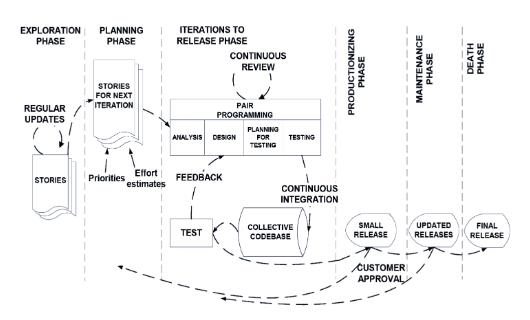
\includegraphics[scale = 0.7]{img/extreme.jpg}
  \caption{Rappresentazione grafica dell'extreme programming}
  \label{extreme}
\end{figure}
\end{document}
% LocalWords:  Machine Learning waterfall png img slides jpg testing self step
% LocalWords:  organizing continuous refactoring Scrum scrum product backlog
% LocalWords:  items dev members owner definzione stakeholders planning daily
% LocalWords:  review retrospective Programming Extreme extreme programming
% LocalWords:  stories Short Releases Metaphor Simple Pair Collective Ownership
% LocalWords:  Integration Customer Coding workspace collective ownership
